\chapter[Resultados]{Experimentos e Resultados}
\label{resultados}
Nesse capítulo, são apresentados detalhes dos experimentos realizados e dos resultados obtidos a partir de simulações utilizando as bases de dados mostradas no \capref{metodologia}.

\section{Análise \textit{dataset DataMining}}  
Na \figref{fig:ResultsMining} tem-se o gráfico da taxa de acerto em função do valor do limiar, o qual foi obtido aplicando o \textit{dataset} proposto por \cite{DataMining} ao \textit{framework}. Para valores de limiar entre 0.8 e 0.84 a taxa de acerto permanece acima de 98.4\%, e conforme o aumento do limiar, além de 0.84, a taxa de acerto vai decrescendo. Tal comportamento é esperado, visto que mesmo um tráfego não malicioso, porém suavemente descorrelacionado do tráfego padrão de referência, seria classificado como um ataque. Nesse sentido, vale ressaltar que existem diferentes tipos de ataques DDoS, os quais geralmente possuem abordagens singulares para a realização dos mesmos. Dessa forma, a escolha de limiares próximos a um não representa uma boa escolha para este tipo de problema, uma vez que a granularidade dos ataques não seria abrangida pelo \textit{framework}. Na tabela \tabref{Tab:ResultsMining} são mostrados  as taxas de acertos, falsos positivos e falsos negativos na análise do \textit{dataset}, complementando o gráfico apresentando na \figref{fig:ResultsMining}.

 \begin{figure}[htb]
 	\centering
 	\caption{Análise do \textit{dataset} \textit{Data Mining} }
 	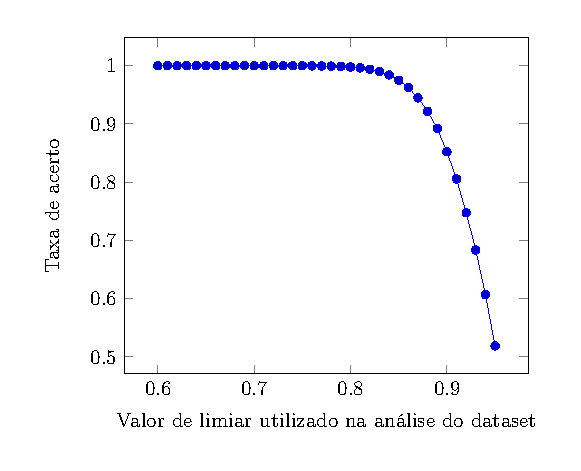
\includegraphics[width=0.9\textwidth]{figs/results80-95Mining.pdf}\\
 	\hspace{1.5cm}{Fonte: Elaborada pelo autor.}
 	\label{fig:ResultsMining}
 \end{figure}
 
 \begin{table}[htb]
 	\centering
 	\begin{threeparttable}
 		\caption{Exemplo base de dados Data Mining}
 		\label{Tab:ResultsMining}
 		%	\small
 		\begin{tabular}{c c c c}
 			\toprule
 			\textbf{Limiar} & \textbf{Taxa de acerto} & \textbf{Taxa de falsos positivos} & \textbf{Taxa de falsos negativos}
 			\\ \midrule
	 			
 			0.60 &  100\% &  NA& 0\%   \\ \midrule
 			0.62 &  99.9996\% &  NA& 0.0003996\%   \\ \midrule
 			0.64 &  99.9996\% &  NA& 0.0003996\%   \\ \midrule
 			0.66 &  99.9996\% &  NA& 0.0003996\%   \\ \midrule
 			0.68 &  99.9996\% &  NA& 0.0003996\%   \\ \midrule
 			0.70 &  99.9992\% &  NA& 0.0007993\%   \\ \midrule
 			0.72 &  99.9992\% &  NA& 0.0007993\%   \\ \midrule
 			0.74 &  99.9992\% &  NA& 0.0007993\%   \\ \midrule
 			0.76 &  99.9800\% &  NA& 0.0.01998\%   \\ \midrule
 			0.78 &  99.9664\% &  NA& 0.03357\%   \\\midrule 		 			 			 			 			 			 			 			
 			0.80 &  99.7790\% &  NA& 0.2210\%   \\ \midrule
 			0.82 &  99.3905\% & NA & 0.6095 \%   \\ \midrule
 			0.84 &  98.4137\%  & NA & 1.5863\%   \\ \midrule
 			0.86 &  96.2556\%  &  NA & 3.7444\%   \\ \midrule
 			0.88 &  92.1842\%  &  NA & 7.8158\%     \\ \midrule
 			0.90 &  85.2309\%  & NA & 14.7691\%    \\ \midrule
 			0.92 &  74.7722\%  &  NA & 25.2278\%   \\ \midrule
 			0.94 &  60.6753\%  & NA & 39.3247\%   \\ \bottomrule
 		\end{tabular}
 		{Fonte: Elaborada pelo autor.}
 	\end{threeparttable}
 \end{table}
Como pode ser visto na tabela \tabref{Tab:ResultsMining}, a coluna "Taxa de falsos positivos" não apresentou nenhuma ocorrência (NA). Esse fato, deve-se especialmente à natureza do \textit{dataset}, o qual é integralmente composto de tráfegos maliciosos e, dessa forma, não se aplica o conceito de falso positivo. Já na coluna "Taxa de falsos negativos"   (tráfego de ataque que foi considerado normal), vemos que dependendo do valor de limiar, temos um número considerável de eventos. Para um valor elevado de limiar, a taxa de acertos baixa e consequentemente, o número de falsos negativos aumenta. 
\section{Análise \textit{dataset} DARPA 2000}
A segunda base de dados usada para avaliar o \textit{framework} é o DARPA, conforme descrito na \capref{metodologia}.
A \figref{fig:ResultsDarpa} apresenta os gráficos das taxas de acertos em função dos limiares simulados. Para limiares entre 0.64 e 0.68, as taxas de acertos ficam entre 60 a 85\%. Tal comportamento é diferente da base de dados anterior, pois as bases diferem em termos de tratamento temporal, modo de detecção e arquivo de respostas, já que no DARPA é mostrada uma janela de tempo onde provavelmente o ataque nomeado irá ocorrer, enquanto no \textit{Datamining} tem-se uma base constituída apenas por ataques. Nesse sentido, espera-se que os valores de taxa de acerto de detecção sejam diferentes para ambos os \textit{datasets}. A \tabref{Tab:ResultsDARPA} mostra as taxas de acertos, falsos positivos e falsos negativos resultantes da análise do \textit{dataset} DARPA 2000. Verifica-se uma baixa taxa de falsos positivos e negativos, tendo em vista que a taxa de detecção é máxima para a maioria dos limiares simulados, mostrando a eficiência do método de detecção.       
 \begin{figure}[htb]
 	\centering
 	\caption{Análise do \textit{dataset} DARPA }
 	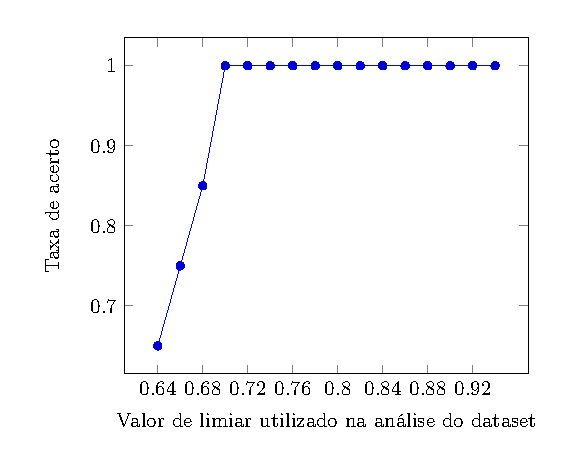
\includegraphics[width=0.85\textwidth]{figs/resultsDarpa.pdf}\\
 	\hspace{1.5cm}{Fonte: Elaborada pelo autor.}
 	\label{fig:ResultsDarpa}
 \end{figure}
 
  \begin{table}[htb]
  	\centering
  	\begin{threeparttable}
  		\caption{Exemplo base de dados DARPA}
  		\label{Tab:ResultsDARPA}
  		%	\small
  		\begin{tabular}{c c c c}
  			\toprule
  			\textbf{Limiar} & \textbf{Taxa de acerto} & \textbf{Taxa de falsos positivos} & \textbf{Taxa de falsos negativos}
  			\\ \midrule
  			0.64 &  65\% &  10\%& 25\%   \\ \midrule
  			0.66 &  75\% & 7.5\% & 17.5 \%   \\ \midrule
  			0.68 &  82.5\%  & 5\% & 12.5\%   \\ \midrule
  			0.70 &  100\%  &  0\% & 0\%   \\ \midrule
  			0.72 &  100\%  &  0\% & 0\%     \\ \midrule
  			0.74 &  100\%  & 0\% & 0\%    \\ \midrule
  			0.76 &  100\%  &  0\% & 0\%   \\ \midrule
  			0.78 &  100\%  &  0\% & 0\%   \\ \midrule
  			0.80 &  100\%  &  0\% & 0\%   \\ \midrule
  			0.82 &  100\%  &  0\% & 0\%   \\ \midrule
  			0.84 &  100\%  &  0\% & 0\%   \\ \midrule
  			0.86 &  100\%  &  0\% & 0\%   \\ \midrule
  			0.88 &  100\%  &  0\% & 0\%   \\ \midrule
  			0.90 &  100\%  &  0\% & 0\%   \\ \midrule
  			0.92 &  100\%  &  0\% & 0\%   \\ \midrule
   			0.94 &  100\%  & 0\% & 0\%   \\ \bottomrule
  		\end{tabular}
  		{Fonte: Elaborada pelo autor.}
  	\end{threeparttable}
  \end{table}
  
 \begin{figure}[htb]
 	\centering
 	\caption{Resultados artigo \cite{HOQUE201748} }
 	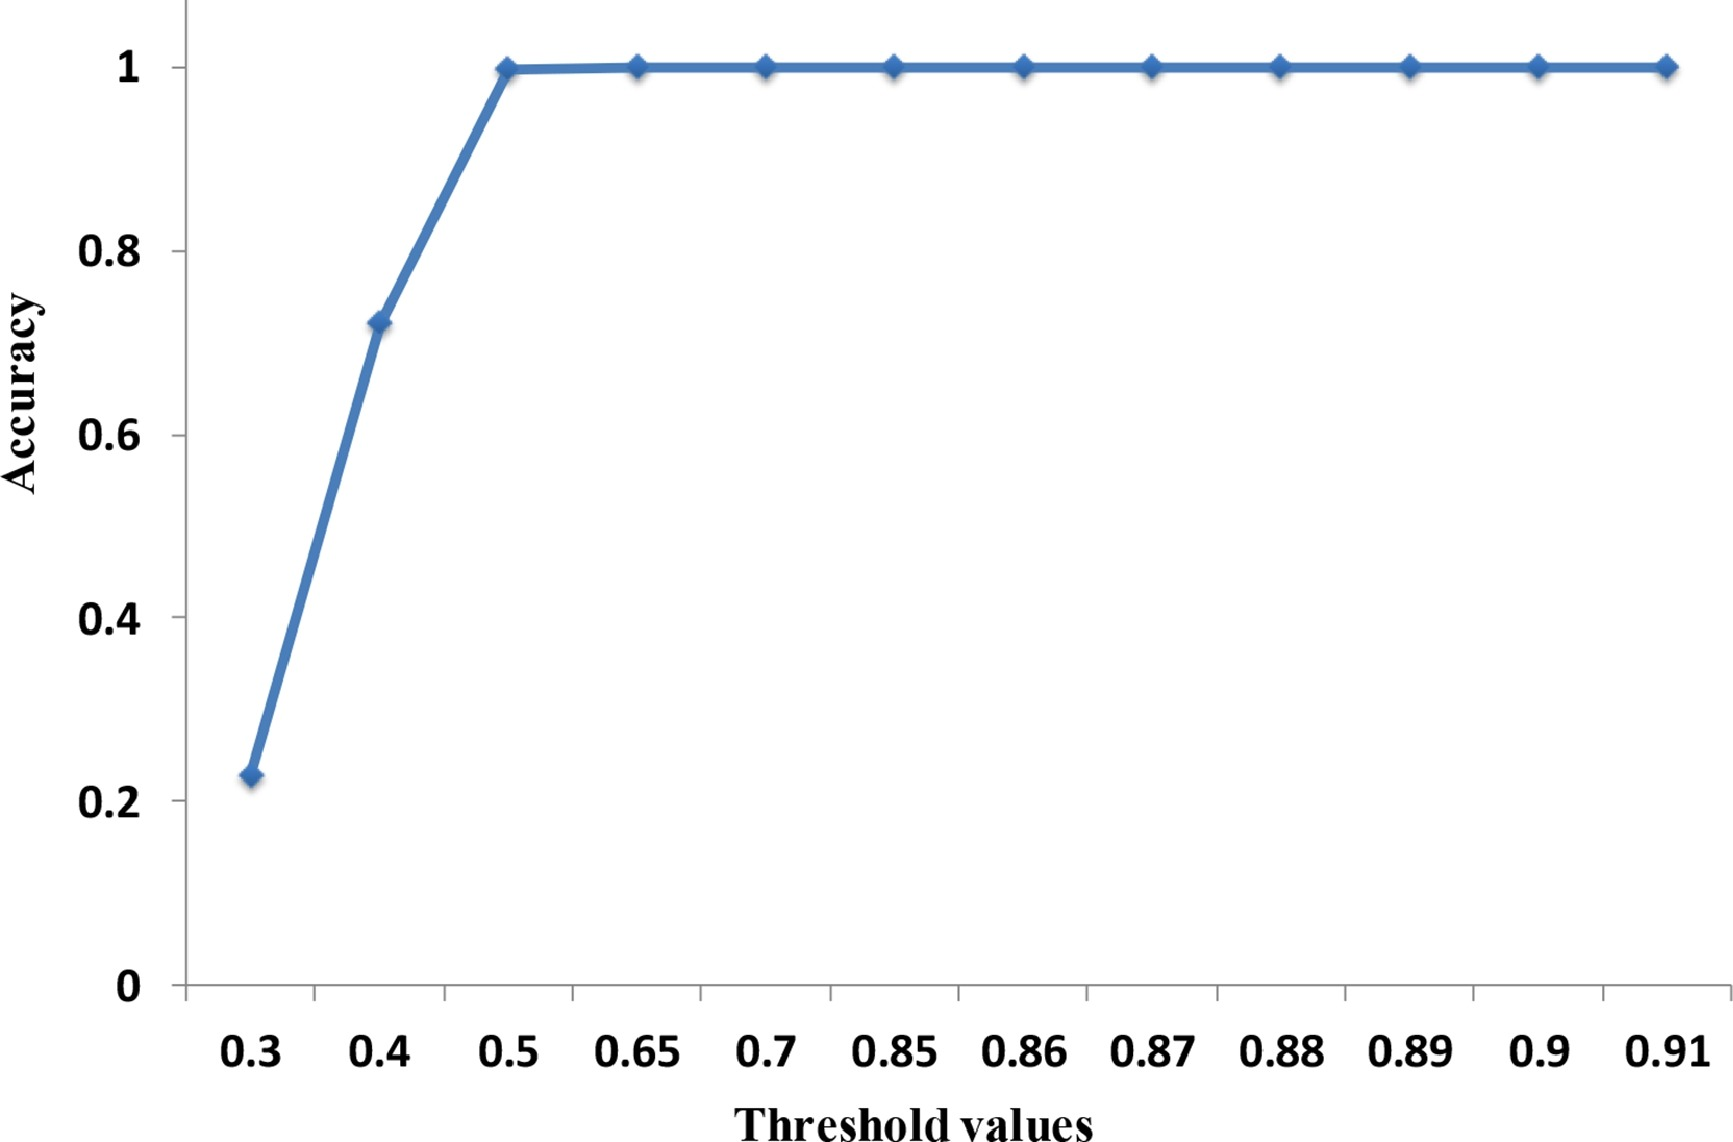
\includegraphics[width=0.7\textwidth]{figs/resultNHOQUE.jpg}\\
 	\hspace{1.5cm}{Fonte: \cite{HOQUE201748}.}
 	\label{fig:ResultsNHOQUE}
 \end{figure}

A \figref{fig:ResultsNHOQUE} mostra os resultados obtidos por \cite{HOQUE201748} para a análise do \textit{dataset} DARPA. Para limiares acima de 70\%, ambos os gráficos têm 100\% de acerto. Assim, ao escolher um intervalo válido de limiares para realizar a detecção deve-se levar em conta os valores para os quais a detecção teve maiores taxas de acerto.

Infelizmente \cite{HOQUE201748} não explicita a versão da base de dados DARPA utilizada em seu trabalho, tampouco respondeu a nossa tentativa de contato por \textit{e-mail}. Portanto, não podemos afirmar categoricamente que usamos a mesma versão do \textit{dataset} DARPA usado por \citeonline{HOQUE201748}. Ao comparar os gráficos resultantes, verificamos grande semelhança em seus valores de taxa de acerto, confirmando que o \textit{framework} implementado está funcionando corretamente.  